\documentclass[../main.tex]{subfiles}

\begin{document}
This section will not cover all of the details of SGX, but only those
applicable to our project; for a complete treatment of SGX please
refer to~\cite{IntelCorporation2010}. \Intel~SGX is a set of x86
instructions that allows for a programming model wherein an
application can be split into two modules: an untrusted component that
executes as normal and a trusted portion that executes within a
protected area of RAM, called an enclave.

The protection of an enclave is managed by the CPU. The CPU
pre-allocates an area of DRAM called the Enclave Page Cache
(EPC)\footnote{This statement is not entirely accurate, the BIOS is
  responsible for allocating an area of memory, called the Processor
  Reserved Memory (PRM), from the which the CPU designates memory for
  the EPC. } where the enclave's data and data strucutres required by
SGX reside in ciphertext form. All data pertaining to an enclave
present in the CPU's caches and registers is held in clear text. Any
data written from the CPU's caches or registers to the EPC is
encrypted first by a memory encryption engine (implemented in
hardware) and is only decrypted when required by the CPU during the
execution of the trusted component, which we refer to as the
\textit{enclave program}, to which that enclave belongs. While the EPC
is shared by all enclaves on the machine, the key used for the
encryption/decryption process is derived from a combination of a
device key, unique to each SGX-enabled CPU, and the ``identity'' of
the enclave (MRENCLAVE), a cryptographic hash of the enclave's
contents at the \textit{enclave program}'s initialization. Moreover
the CPU performs a series of checks to ensure that no process, other
than the one that initialized the enclave, may access the protected
area in DRAM.

Interacting with the \textit{enclave program}, as a result, may only
occur through invoking a programmer defined interface, called a
callgate, as depicted in Figure~\ref{fig:sgxhighlevel}.

\begin{figure}[H]
  \centering
  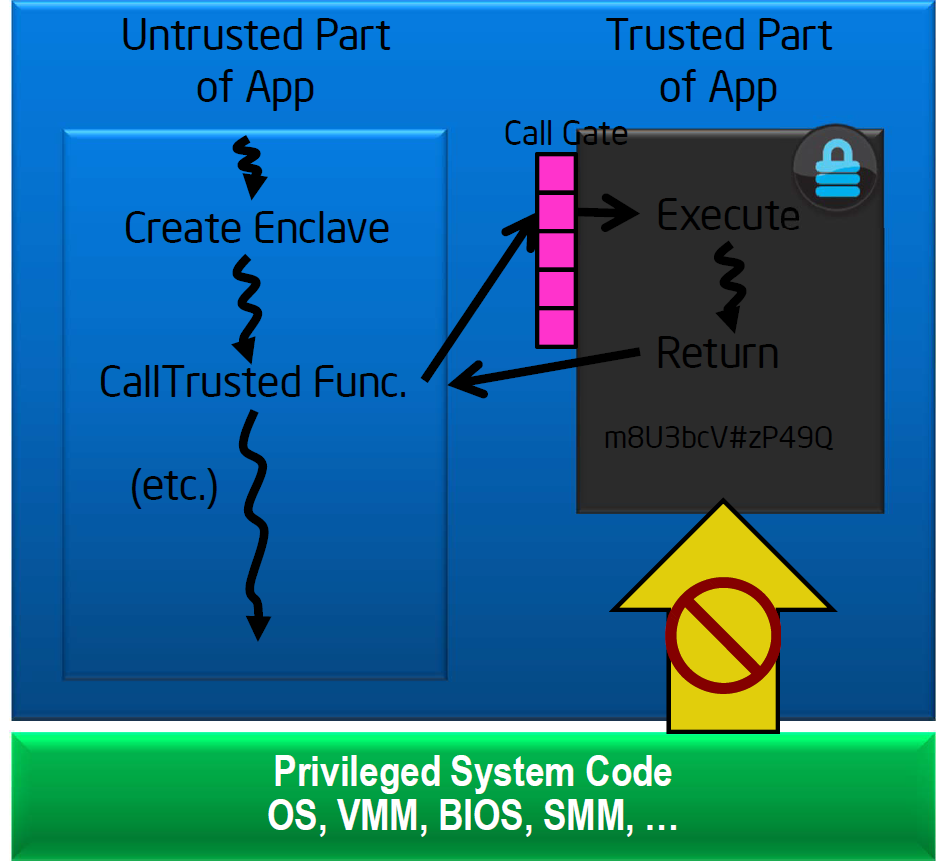
\includegraphics[scale=0.25]{images/sgxhighlevel.png}
  \caption{Interaction of the untrusted part of the application with
    the trusted part can only occur through a
    callgate~\cite{IntelCorporation2010}}
  \label{fig:sgxhighlevel}
\end{figure}

\subsubsection{Initialising an SGX Enclave}

Launching an SGX \textit{enclave program} requires the execution of
the following steps:

\begin{enumerate}
  \item The \textit{enclave program} is first compiled and then signed
    by a private key that corresponds to an \Intel~ verified certificate.
    While the requirements imposed on the certificate for successful
    verification are well documented, the process is not automated, and
    involves an application to \Intel's Infrastructure Attestation Service
    (IAS). This implies that \Intel~could arbitrarily deny software
    developers the abillity to launch SGX code.The signing process
    generates a data structure called \texttt{SIGSTRUCT} that contains the
    aforementioned MRENCLAVE, the identity of the signing entity,
    MRSIGNER, and the signature across this structure.
  \item When attempting to launch the \textit{enclave program}, the
    CPU calculates MRENCLAVE using privileged SGX instructions, calculates
    MRSIGNER by taking the hash of the public key contained in the signing
    entity's certificate, and then attempts to verify that
    MRSIGNER$_{calc}$ is equal to MRSIGNER$_{SIGSTRUCT}$,
    MRENCLAVE$_{calc}$ is equal to MRENCLAVE$_{SIGSTRUCT}$, and that the
    signature across \texttt{SIGSTRUCT} was generated by the signing
    entity indicated by MRSIGNER.
  \item If all previous checks complete successfully, then the CPU
    proceeds to execute the \textit{enclave program}, otherwise, the CPU
    aborts execution.
\end{enumerate}

In using SGX, however, one trusts \Intel~ not only to implement SGX
correctly, otherwise an enclave may be compromised due to
vulnerabilities, but also not to introduce trapdoors into SGX (not all
of SGX's details are public knowledge, yet) that could allow them to
compromise an enclave. Nevertheless, for the purposes of this report,
we find that it is reasonable to trust \Intel~ seeing as their CPUs
are in use by many cloud-providers.

Moreover, SGX has gained momentum as a research platform for security
related work such as Haven~\cite{Baumann14}, which secures a legacy
application from a non-trusted OS and cloud-provider \textit{without}
modifying the application's source code. Yet, there is no work, to our
knowledge, that attempts to secure only the private key material
through use of SGX. Narrowing the trusted region to contain only the
component that handles the private key allows us to define a much
smaller trusted computing base that only contains the CPU and the code
that handles the long-term private key. This also means that the
memory footprint of the \textit{enclave program} in our design is
smaller than that of Haven's, making it easier to fit our memory in
the EPC which is set to a static size of ~90MB on machines that
currently support SGX

At the time we begun working on this project we could not obtain
access to SGX hardware, forcing us to use a simulator. There were two
choices: OpenSGX and the \Intel~ Windows SDK's simulation
mode. We selected the former to implement our prototype as it was
compatible with Linux, a platform we were more familiar with, and had
several examples we could refer to for guidance in our implementation
(the Intel SDK, at the time, was under-documented). The following
section provides a quick examination of OpenSGX's salient features.


\subsubsection{Brief Notes on OpenSGX}
\subfile{sections/opensgx.tex}
\end{document}

%%% Local Variables:
%%% mode: latex
%%% TeX-master: "../main"
%%% End:
